\chapter{Error Analysis via Simulation}\label{ch:simulation}
There are many factors impacts the accuracy in UAS localization and 
feature position estimation, and they can be sorted into three main 
categories: 

\begin{enumerate}
  \item Noise in system intrinsic parameters. The system intrinsic
  parameters includes
  \begin{itemize}
    \item Camera intrinsic parameters
    \begin{itemize}
      \item Coordinate of optical center on image plane $[c_{x}, c_{y}]$
      \item Scaling factor to project feature in 3D world to image
      plane $ [f_{x}, f_{y}]$
      \item Lens distortion parameters $[k_{1}, k_{2}, p_{1}, p_{2}]$
    \end{itemize}
    \item Image resolution.
    \item Accelerometer bias 
  \end{itemize}
  \item Error introduced by LK tracking algorithm. Reliable vision
  tracking is an entire field of research in itself. Pyramid
  implementation of Lucas-Kanade (LK) tracking is used in this work,
  and there are a number of factors contribute to its performance.
  Firstly, LK tracking algorithm tracks features by comparing the
  intensity of a window of the image centered at the feature
  coordinate in image from one frame to another. The searching process
  terminates when the sum of error on the windowed image intensity is
  lower than a value set by user, or when iteration of search has
  reached a maximum number set by user. Secondly, as scene evolve from
  frame to frame, the initial feature appears differently from frame
  to frame as the viewing distance and angle is different. Thirdly,
  sudden intensity change in the image sequences significant noise in
  the tracking. In outdoor setting, intensity change can be introduced
  by many factors, such as changes of sky area in a image, sun glare,
  UAV enters or exits cloud shades, or camera auto-adjust its shuttle
  speed, etc.
  \item Error caused by the SLAM algorithm itself. The algorithm
  estimated features coordinate through a model that represents the
  relation between UAS location, feature location and UAS motion. As
  the model is non-linear, the linearization process introduces error
  into the result.
\end{enumerate}

To better understand the impact of the factors listed above. A 
simulation is performed to examine the impact item 1 and item 3. 

The simulator first generates a 3D point cloud ranging from 100 meters
to 3000 meters from the camera (Figure \ref{fig:simfig51}). At each
frame, the coordinates of the 3D points are first transformed to the
new camera frame using the measured UAS motion. Next, the 3D points
are projected to the image plane using a camera model defined by
$[c_{x}, c_{y}, f_{x}, f_{y}, k_{1}, k_{2}, p_{1}, p_{2}]$, and
digitized to a resolution of choice.

\begin{figure}[h]
\centering
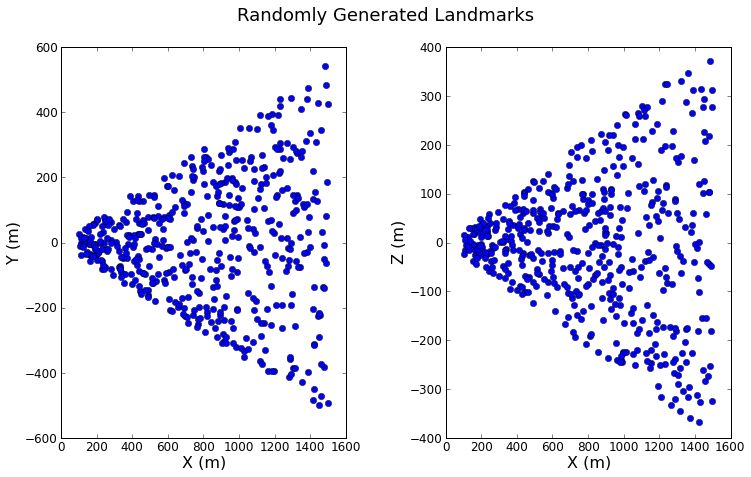
\includegraphics[width=12cm, height=7cm]{./Figures/SimulationFigures/Figure51.png}
\caption{Randomly Generated 3D Feature Points}
\label{fig:simfig51}
\end{figure}

\section{An Ideal Case}
First of all, understanding the algorithm's performance under no noise, 
or nearly no noise condition provide a solid ground for the analysis 
later on. This simulation shows how much error the model itself 
generates under the most basic flying condition, which is moving forward 
at constant speed. The low noise environment is configure as such,

\begin{itemize}
  \item UAS is moving forward (X axis) with constant speed at 60 knots. 
  \item Y axis and Z axis translational movement are limited to white
  noise with standard deviation of 0.08 meters and a mean of 0.
  \item UAS rotation are modelled by white noise with standard
  deviation of 0.01 degree and a mean of 0
  \item No error was introduced due to image digitization. (i.e. the
  projected feature position on image plane was not digitized to any
  sensor resolution)
  \item No error was introduced from camera model mismatch. (i.e.
  camera model used by simulator is exactly the same as the one used
  by CC\_EKF\_SLAM algorithm.
\end{itemize}

\subsection{UAS Localization}
The estimation of UAS coordinate and orientation is first analyzed, as 
these estimates are directly used to perform transformation between 
camera and world frame. Figure \ref{fig:simfig1} plots the UAS 
translation and rotation against video frame number. The ground truth 
and estimated value are plotted in blue and green lines respectively. 
The error defined by $Estimated-Ground Truth$ is plotted in red line. 
Under a simple forward only motion, the algorithm tracked the UAS status 
quite well, with error on translational motion less than 1 cm and error 
on rotational motion less than 3e-3 degree. 

\begin{figure}[h]
\centering
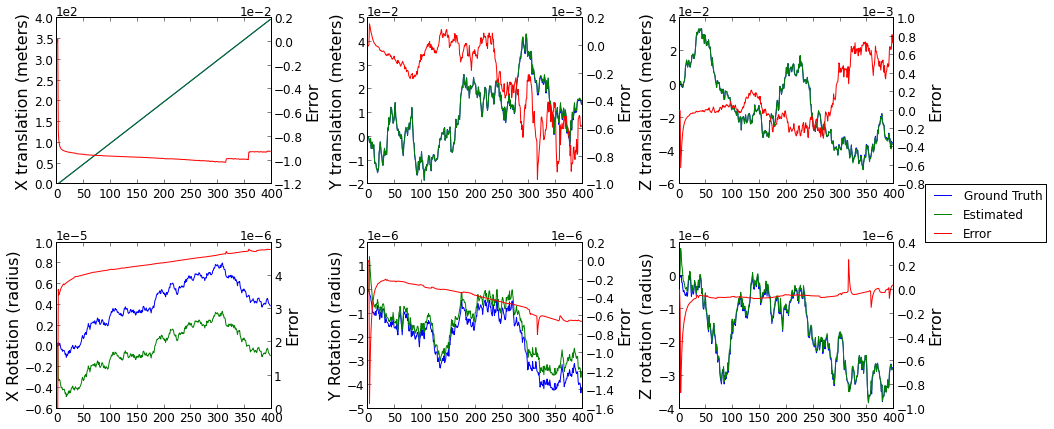
\includegraphics[width=15cm, height=7cm]{./Figures/SimulationFigures/Figure1.png}
\caption{UAS localization error under no noise condition}
\label{fig:simfig1}
\end{figure}


\subsection{Features Mapping - Convergence and Accuracy}

Figure \ref{fig:simfig5-8} left shows feature parameters $[d, \varphi
,\theta]$ (where $d=1/\rho $) plotted against frame number for the
first 50 frames. The feature depth $d$ for all features converged
within 3 frames; elevation-azimuth angles $[\varphi ,\theta]$ stay
almost constant after initialization. A more detail graph can be seen
from the error convergence plot for these parameters (Figure
\ref{fig:simfig5-8} right.) which shows the tracking error of these
parameters for 400 frames. The error of feature distance$ d$ continues
to approach zero as the tracking continues. $[\varphi ,\theta]$ show
small drift within $+/-0.0002^{\circ}$ respectively. However, as
tracking continue into later frames, error of $[\varphi ,\theta]$
gradually grew bigger. The resulting error for feature coordinate in
world frame represented in standard Euclidean XYZ parameterization is
plotted in ??. The features positions errors in world frame converge
to zero as tracking continues. During the process, certain features
moved out of the FOV, and therefore its position estimation remained
unchanged since then. At the end of the 400 frames, the x axis
position error of the feature reduced to +/-0.2 meters; y and z axis
error reduce to +/-0.02 meters

\begin{figure}[h]
\centering
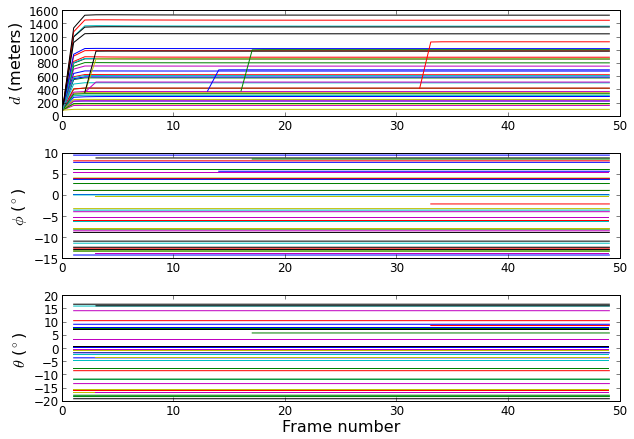
\includegraphics[width=7cm, height=5cm]{./Figures/SimulationFigures/Figure6.png}
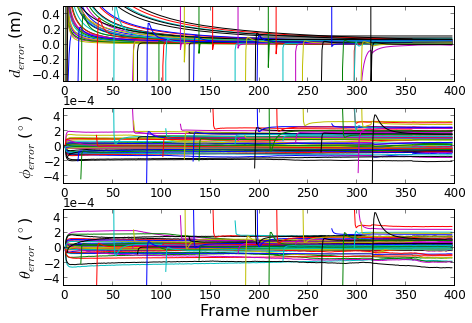
\includegraphics[width=7cm, height=5cm]{./Figures/SimulationFigures/Figure7.png}
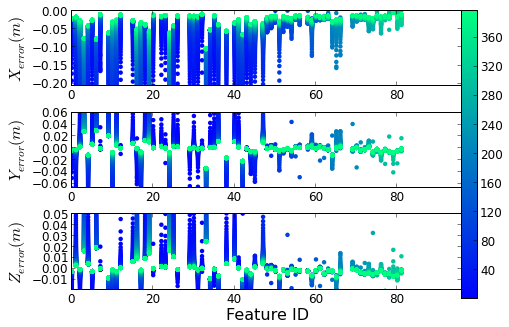
\includegraphics[width=7cm, height=5cm]{./Figures/SimulationFigures/Figure5.png}
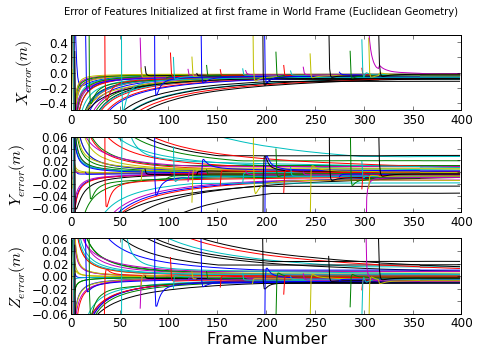
\includegraphics[width=7cm, height=5cm]{./Figures/SimulationFigures/Figure8.png}
\caption{Features parameters and error convergence under no noise condition}
\label{fig:simfig5-8}
\end{figure}

\section{Effect of UAS Motion}

The simulation result from UAS forward travel shows that the 
CC\_EKF\_SLAM algorithm does feature tracking and self localization 
quite well under simple UAS motion. Next, the algorithm is tested with a 
more complex and realistic scenario. A series of motion is added to the 
simulation in addition to the forward motion. The remaining 5 types of 
maneuver are added one at a time. These maneuvers are: translation on Y, 
translation on Z, rotation on X, rotation on Y and rotation on Z. Each 
motion is modelled by a sine wave with frequency at 1Hz, and variable 
amplitude. For translation on Y and Z axis, the sine amplitude varies 
from 1 meter to 19 meters with 2 meters increments. For X, Y, and Z axis 
rotation, the amplitude varies from 0.001 radius to 0.018 radius with 
0.001 radius increment. 

\subsection{UAS Localization under Motion}

Figure \ref{fig:simfig9-10} shows the UAS localization error statistic
under translation motion on Y and Z axis and rotation motion on X, Y,
and Z axis. The blue dots mark the mean value $\mu$ of the error
throughout the tracking, and the error bars mark the standard
deviation $\sigma$.

The translation motion clearly increases the error of UAS localization. 
However, the amount of increase is insignificant. With the Sine 
amplitude increased to 19m, UAS position error increased by less than 
0.02 meter. 

On the other hand, rotation motions have a big impact on the accuracy of 
localization. Rotation on X axis has small effect on the accuracy of UAS 
position and orientation estimate. No obvious increase on mean and 
standard deviation of the error can be observed. Rotations on Y and Z 
axis yield significant error increase on the position of the UAS. 

\begin{itemize}
  \item Rotation on Y axis increases the UAS X position mean error, as
  well as the standard deviation. For Z positioning of the UAS, the
  mean error stays zero, but standard deviation increase dramatically.
  \item Same thing happens to the X and Y positioning for rotation on
  Z axis.
\end{itemize}

\begin{figure}[h]
  \centering
  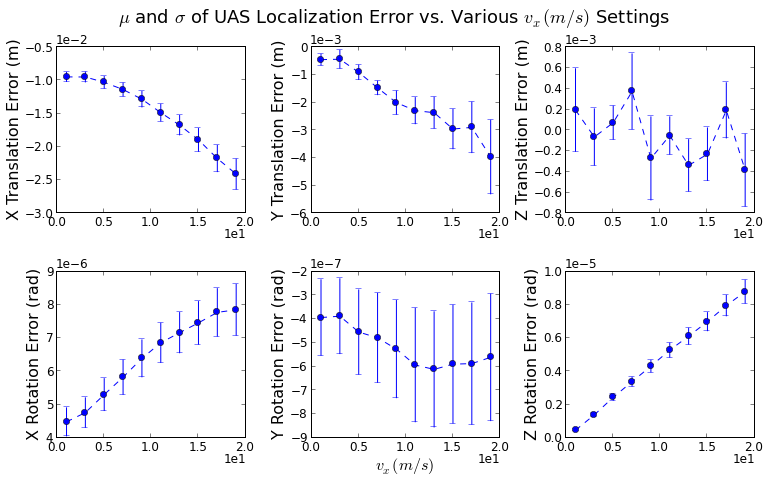
\includegraphics[width=4.5cm, keepaspectratio=true]{./Figures/SimulationFigures/Figure9.png}
  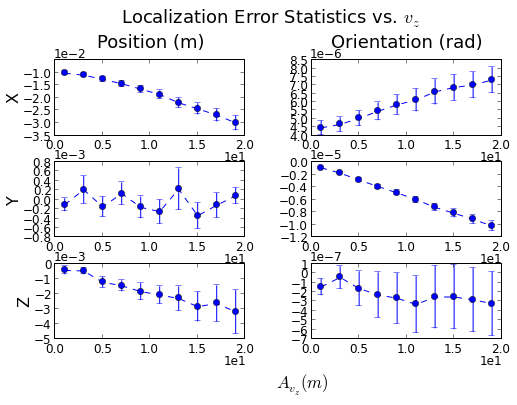
\includegraphics[width=4.5cm, keepaspectratio=true]{./Figures/SimulationFigures/Figure10.png}
  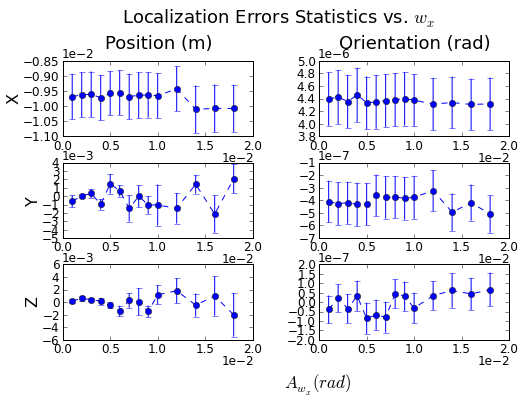
\includegraphics[width=4.5cm, keepaspectratio=true]{./Figures/SimulationFigures/Figure11.png}
  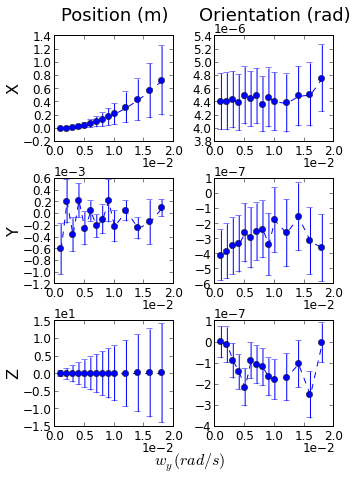
\includegraphics[width=4.5cm, keepaspectratio=true]{./Figures/SimulationFigures/Figure12.png}
  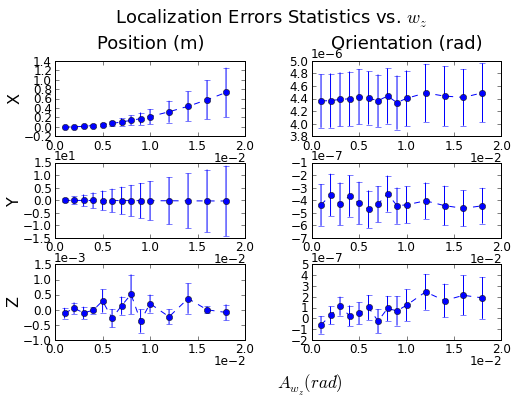
\includegraphics[width=4.5cm, keepaspectratio=true]{./Figures/SimulationFigures/Figure13.png}
  \caption{UAS localization error under translational 
  \label{fig:simfig9-10}
    motion}
  
\end{figure}

To understand how rotation motion affect the UAS localization
estimation, the UAS position on X, Y, Z in world frame are plotted
below (figure \ref{fig:simfig14}) with rotation amplitude on X, Y and
Z set at 0.01 radius. With rotation on X axis, the position error of
UAS shows some oscillation. The oscillation magnitude remains small
(in the scale of millimeters) and around zero. For rotation on Y and
Z, the situation is very different. Both rotation motions caused the
UAS position error to oscillate with the oscillation amplitude
increasing (diverging) as tracking goes on. The X position error of
the UAS increases in positive value with both rotation on Y and Z, but
the most significant impact happens on the Z position (for rotation on
Y) and Y position (for rotation on Z), with error reaching 20 meters
at the end of the video sequence. With rotation rate increases
(amplitude of the sine wave), the rate of error diverging from zero
also increases, hence, resulting in an increasing error standard
deviation in error statistic plots. This simulation result suggests
that CC\_EKF\_SLAM algorithm is very sensitive to rotation on Y and Z
axis.

\begin{figure}[h]
  \centering
  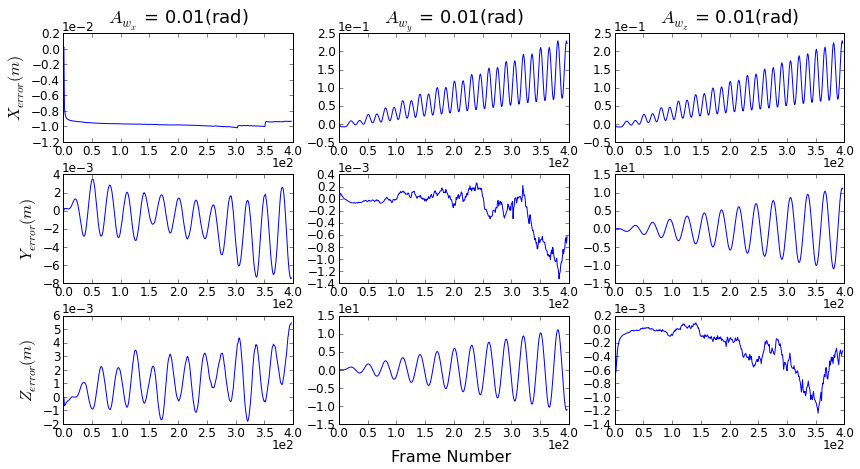
\includegraphics[width=14cm, keepaspectratio=true]{./Figures/SimulationFigures/Figure14.png}
  \caption{UAS estimated position in world frame}
  \label{fig:simfig14}
\end{figure}

\subsection{Feature Mapping Accuracy under Motion}

Feature mapping error statistic are drawn from the feature error at
last frame, since features error converge to zero as tracking goes on.
Figure \ref{fig:simfig20-24} shows the feature mapping error statistic
with added motions. Translation motions increase both the error mean
and standard deviation, but not by much. With the motion maximum
amplitude ranging from 1 meters to 19 meters, the increases of
features position error mean and standard deviation are both in the
scale of centimeters.

\begin{figure}[h]
  \centering
  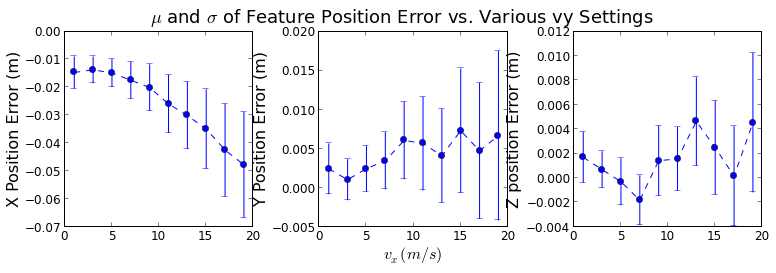
\includegraphics[width=7cm, height=2.5cm]{./Figures/SimulationFigures/Figure20.png}
  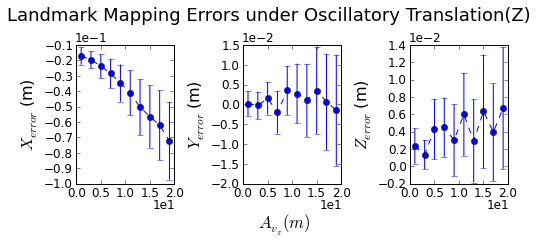
\includegraphics[width=7cm, height=2.5cm]{./Figures/SimulationFigures/Figure21.png}
  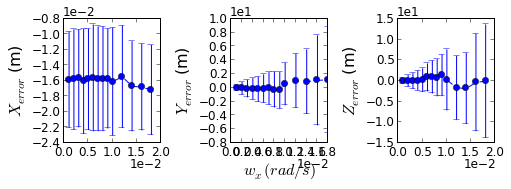
\includegraphics[width=7cm, height=2.5cm]{./Figures/SimulationFigures/Figure22.png}
  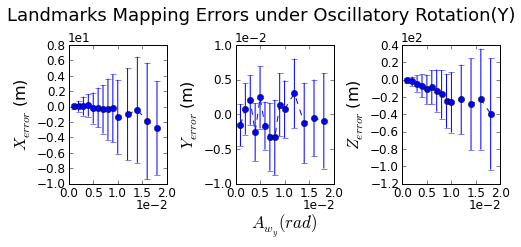
\includegraphics[width=7cm, height=2.5cm]{./Figures/SimulationFigures/Figure23.png}
  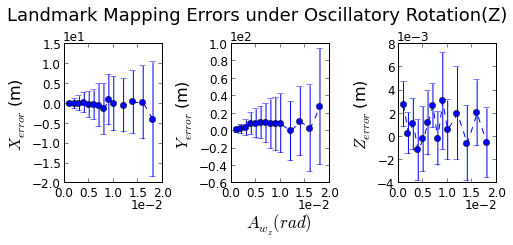
\includegraphics[width=7cm, height=2.5cm]{./Figures/SimulationFigures/Figure24.png}
  \caption{Feature mapping error under added motion}
  \label{fig:simfig20-24}
\end{figure}

With maximum rate of rotation ranging from 0.001 rad/frame to 0.018
rad/frame

\begin{itemize}
  \item Rotation on all three axis yields significant error increase
  for feature position estimation
  \item X axis rotation causes increase on standard deviation of Y and
  Z axis feature position error, and by similar amount. The error are
  in scale of meters with maximum rotation setting.
  \item Y axis rotation causes increase on mean and standard deviation
  of X and Z axis feature position error. Z axis feature position
  receives the biggest impact with error in the scale of hundreds of
  meters with maximum rotation setting
  \item Z axis rotation impacts on X and Y axis feature position in a
  similar way as the Y axis rotation.
\end{itemize}

\begin{figure}[h]
  \centering
  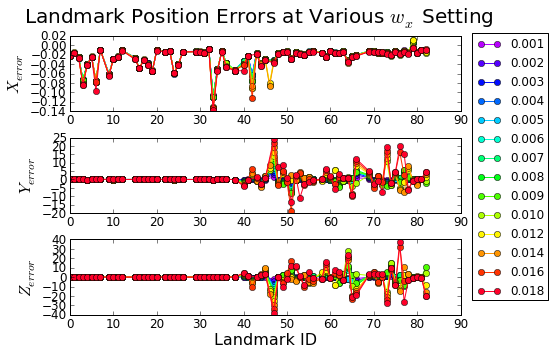
\includegraphics[width=7cm, height=5cm]{./Figures/SimulationFigures/Figure17.png}
  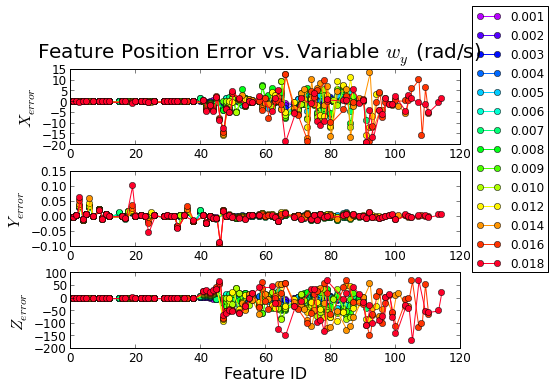
\includegraphics[width=7cm, height=5cm]{./Figures/SimulationFigures/Figure18.png}
  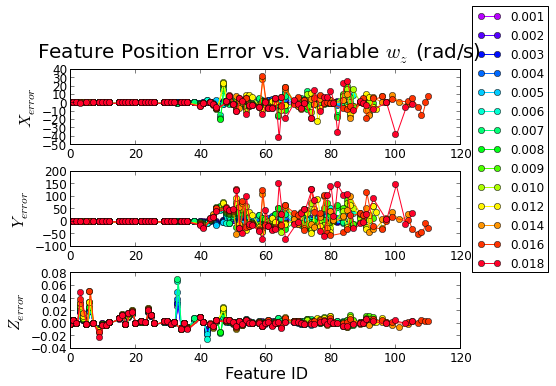
\includegraphics[width=7cm, height=5cm]{./Figures/SimulationFigures/Figure19.png}
  \caption{Feature mapping error under rotatioanl motion}
  \label{fig:simfig17-19}
\end{figure}

Figure \ref{fig:simfig17-19} shows the features position error at the last
tracking frame for all three type of rotation motion. The errors are
plotted against feature ID and it revealed some more characteristic of
the features mapping errors.

\begin{itemize}
  \item With rotation on Y and Z, the tracked features easily went out
  of FOV. This can be observed from total number of features went from
  80 to over 110 with Y axis rotation setting varied from 0.001rad/s
  to 0.018rad/s. This caused frequent addition of new features.
  \item Features added after first frame has much bigger error than
  features added at first frame. At 1$^{st}$ frame, 40 features added
  to the filter. Error plots from Y and Z axis rotation both shows
  that major feature mapping error came from features added after the
  1 $^{st}$ frame with ID bigger than 40.
\end{itemize}

To investigate how does rotation motion results in bigger error on
features added after first frame, feature parameters error (converted
to world frame) with $wy = 0.01$ are plotted in
figure \ref{fig:simfig25}. It is found that the most significant
error happen to parameter $\phi$ which is the feature elevation angle.
This angle has the same definition as rotation angle around Y axis.
The second contributor is $z_i$ (the Z axis coordinate of the feature
initialization point). The both parameters have an offset error at
initialization, and were never corrected throughout the tracking.

Figure \ref{fig:simfig26} shows the $\phi$ error at 
initialization in camera frame and world frame. The blue line shows the 
error in camera frame. The red line shows the error in world frame 
transformed using the estimated UAS position and orientation. It is 
clear that it is the transformation process that introduced the offset 
error in $\phi$. Offset error in $z_i$ is due to the same 
reason. Recall that with Y axis rotation, UAS localization estimate has 
biggest error in X and Z axis coordinates estimate. Features initialized 
at first frame don't carry any offset error is because the 
transformation process is using the same parameters in both way. During 
tracking, these features are transformed to the new camera frame using 
the estimated UAS position and orientation. These are the same 
estimation being used to transform feature position from camera frame 
into world frame. Therefore, although the UAS localization estimations 
are different from the ground truth, feature initialized at first frame 
were not affected. To conclude, the major contributor for feature 
mapping error came from error in UAS localization estimation.

\begin{figure}[h]
  \centering
  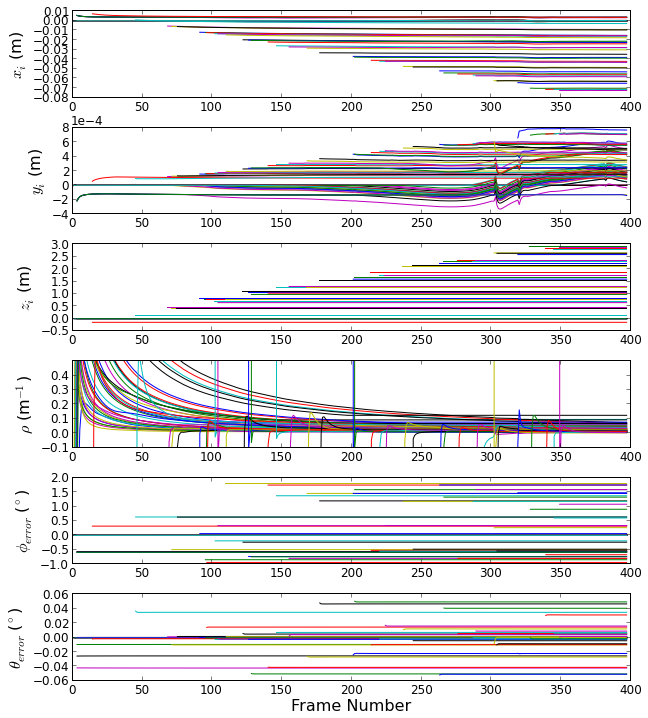
\includegraphics[width=10cm, height=12cm]{./Figures/SimulationFigures/Figure25.png}
  \caption{Feature parameters error under rotatioanl motion}
  \label{fig:simfig25}
\end{figure}

\begin{figure}[h]
  \centering
  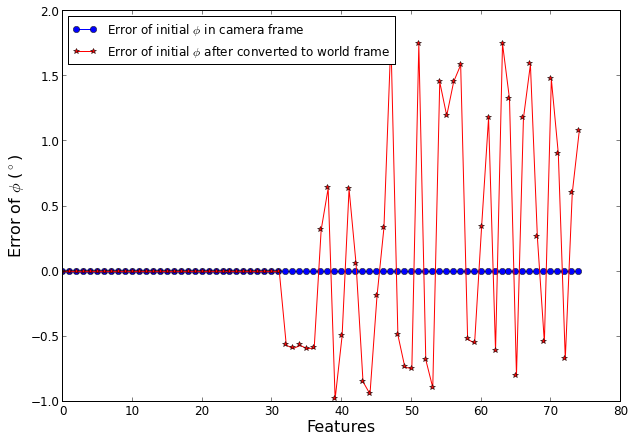
\includegraphics[width=10cm, height=7cm]{./Figures/SimulationFigures/Figure26.png}
  \caption{Error of $\phi$ in camera frame and world frame at initialization}
  \label{fig:simfig26}
\end{figure}

\FloatBarrier
\section{Camera Intrinsic Parameters}
This section summarizes the impact of inaccurate camera parameters 
estimations. Error on camera intrinsic parameters is simulated by using 
different values for camera models. One model is used in the simulator 
to project 3D points onto image plane, and the other is used in the 
measurement model of CC-LK-SLAM. $c_{x}$, $c_{y}$, $f_{x}$, and 
$f_{y}$ are simulated individually and distortion parameters $[k1, 
k2, p1, p2]$ are simulated as a group. Using the calibrated camera 
model (see section ???) as a base model,$ c_{x}$, $c_{y}$, $f_{x}
$, and $f_{y}$ in simulator camera model varied from -50\% to 50\% of 
the base model. Distortion parameters varied from 0\% to 140\% of the 
base model. 

\subsection{Effect from $(c_{x}, c_{y})$}

Figure \ref{fig:simfig34-35} show an over view of UAS localization
error statistics with incorrect estimates of $ (c_{x}, c_{y})$.

\begin{figure}[h]
  \centering
  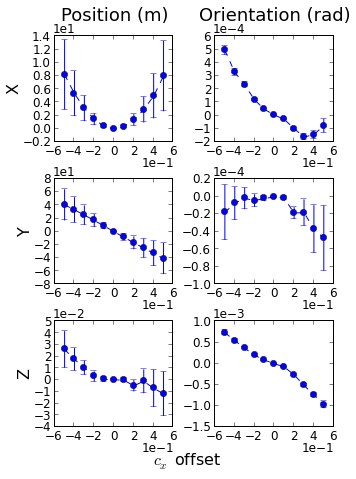
\includegraphics[width=5cm, keepaspectratio=true]{./Figures/SimulationFigures/Figure34.png}
  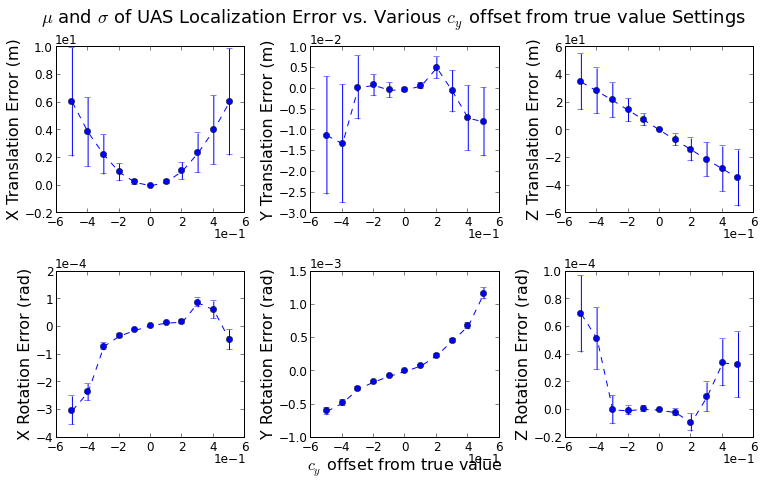
\includegraphics[width=5cm, keepaspectratio=true]{./Figures/SimulationFigures/Figure35.png}
  \caption{UAS localization error statistic with varying $(c_x, c_y)$}
  \label{fig:simfig34-35}
\end{figure}

UAS position error is dependent on $(c_{x}, c_{y})$ and time (figure
\ref{fig:simfig36-37}). The UAS position error is diverging (increases
in time), and can be modeled by 1 $^{st}$ order polynomial function,
with the rate of diverging decided by the error of $(c_{x}, c_{y})$.
$c_{x}$ affects UAS position on X and Y axis, and $c_{y}$ affects UAS
position on X and Z axis.

\begin{figure}[h]
  \centering
  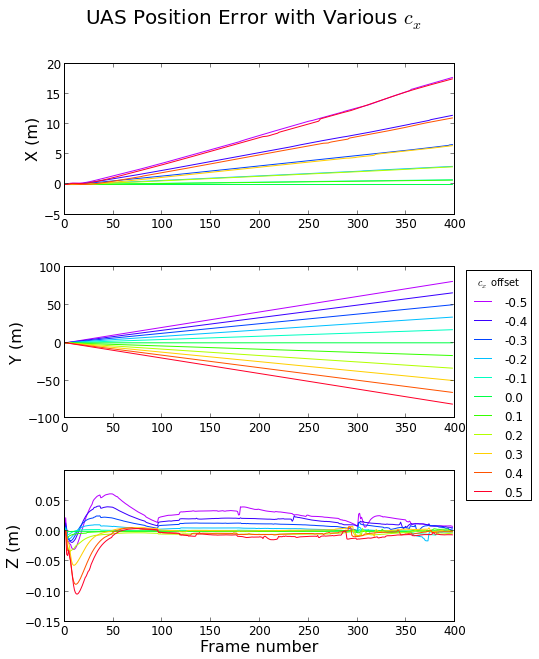
\includegraphics[width=7cm,keepaspectratio=true]{./Figures/SimulationFigures/Figure36.png}
  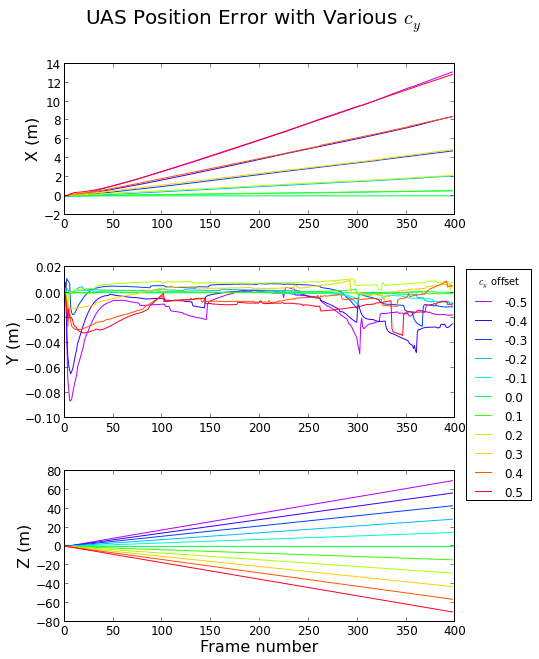
\includegraphics[width=7cm,keepaspectratio=true]{./Figures/SimulationFigures/Figure37.png}
  \caption{Diverging UAS position error}
  \label{fig:simfig36-37}
\end{figure}

The feature mapping error statistics from incorrect estimate of $
(c_{x}, c_{y})$ are plotted in figure \ref{fig:simfig28-29}. The
following characters can be observed from the plots:

\begin{itemize}
  \item Incorrect $c_{x}$ affect feature position on all axis, among
  which, X and Y axis see the most significant error.
  \begin{itemize}
    \item The further $c_{x}$ deviate from the true value, the further
    the features appear (positive X axis error).
    \item On Y axis, smaller $c_{x}$ make feature appear further to
    the optical axis than ground truth (positive error), and bigger
    $c_{x}$ make features appear closer (negative error).
    \item Incorrect $c_{x}$ also affect Z axis feature position, but
    by a much smaller amount.
  \end{itemize}
  \item Incorrect $c_{y}$ affect feature position on all axis
  similarly to $c_{x}$. Estimates on X and Z axis show most amount of
  error.
\end{itemize}

\begin{figure}[h]
  \centering
  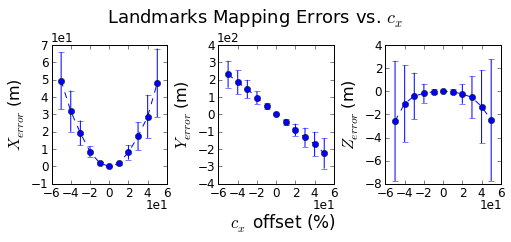
\includegraphics[width=5cm, keepaspectratio=true]{./Figures/SimulationFigures/Figure28.png}
  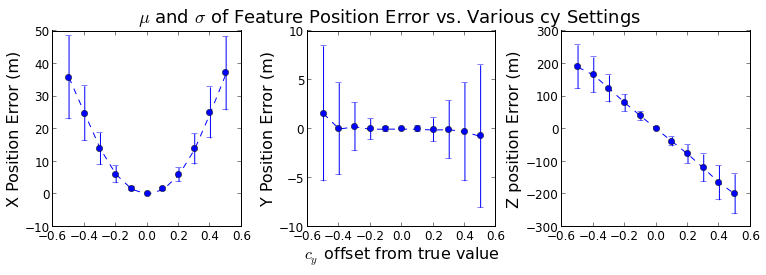
\includegraphics[width=5cm, keepaspectratio=true]{./Figures/SimulationFigures/Figure29.png}
  \caption{Feature mapping error statistic with varying $(c_x, c_y)$}
  \label{fig:simfig28-29}
\end{figure}

Plotting feature position error as a function of features ground truth 
positions reveals more information on how incorrect $c_{x}$ and $
c_{y}$ affect feature mapping. Feature position error is a function of 
its ground truth position, and $c_{x}$ (or $c_{y}$). 

\begin{itemize}
  \item Error on X axis is proportional to the ground truth position
  on X. The further the feature is, greater the error. The degree of
  incorrectness in $c_{x}$ decide the slope of the error plot, greater
  the error in $c_{x}$, steeper the slope (figure
  \ref{fig:simfig32-33}, plot (a), subplot $[1,1]$).
  \item Feature position error on Y axis is also proportional to the
  ground truth position on X with the slope polarity dependent on the
  polarity of the error of $c_{x}$, and error plot slope dependent on
  the error of $c_{x}$.
  \item Feature position error on Z axis is proportional to the ground
  truth position on Z, with slope polarity dependent on the polarity
  of error of $c_{x}$, and slope dependent on the error of $c_{x}$.
\end{itemize}

$c_{y}$ affects feature position similarly to $c_{x}$ (figure
\ref{fig:simfig32-33}, plot (b)), except feature position error on Z
is dependent on ground truth position on X, and error on Y is
dependent on the ground truth position on Y.

\begin{figure}[h]
  \centering
  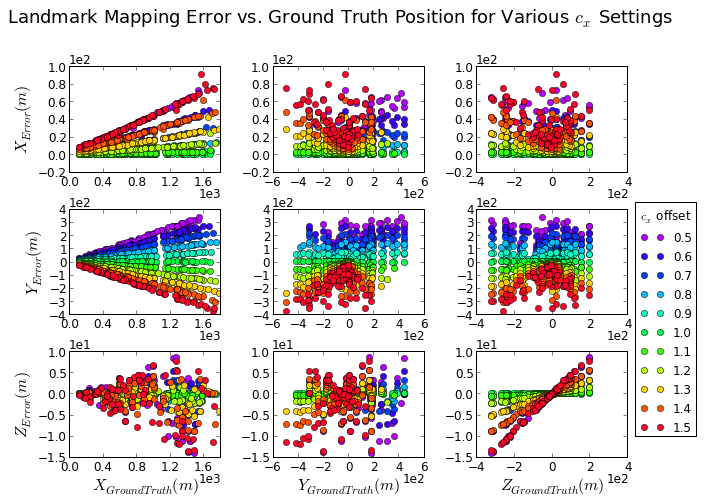
\includegraphics[width=7cm, height=5cm]{./Figures/SimulationFigures/Figure32.png}
  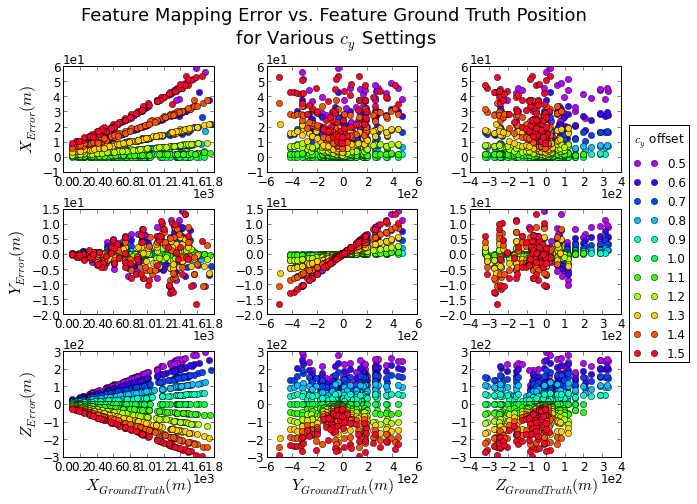
\includegraphics[width=7cm, height=5cm]{./Figures/SimulationFigures/Figure33.png}
  \caption{Feature mapping error vs. ground truth feature position}
  \label{fig:simfig32-33}
\end{figure}

\FloatBarrier
\subsection{Effect from $(f_x, f_y)$}

With $(f_x, f_y)$ varying from -50\% to +50\% of the calibrated
value, the UAS localization error is shown in \ref{fig:simfig43-44}.
For all $f_x$ and $f_y$ settings, UAS position error remained less than
+/-0.05 meters, and orientation error remained in less than 8e-6
radius. Compared to the error obtained from the ideal case simulation,
Error in $(f_x, f_y)$ estimation does not introduce any additional error into
UAS localization estimate. 
\begin{figure}[h]
  \centering
  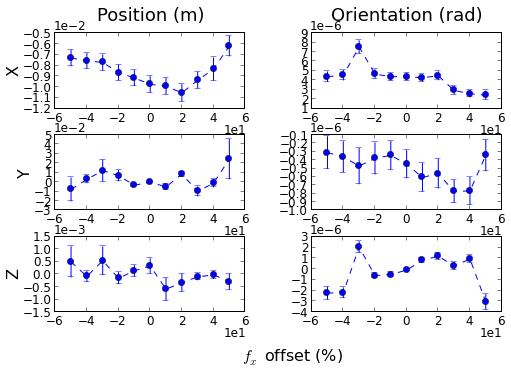
\includegraphics[width=5cm,keepaspectratio=true]{./Figures/SimulationFigures/Figure43.png}
  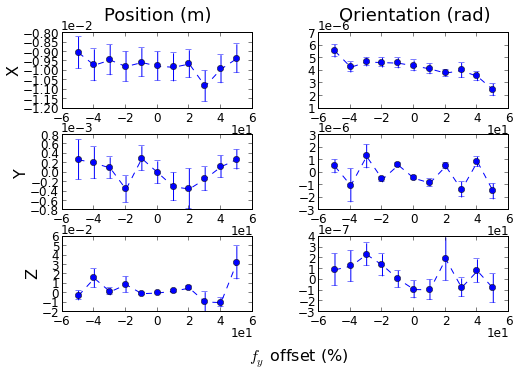
\includegraphics[width=5cm,keepaspectratio=true]{./Figures/SimulationFigures/Figure44.png}
  \caption{UAS localization error statistic with variable $(f_x, f_y)$}
  \label{fig:simfig43-44}
\end{figure}

Feature mapping, on the other hand, is unavoidably affected by the error
in $(f_x, f_y)$ since these are the scaling factor that project
features from 3D world onto image plane. Figure \ref{fig:simfig38-39}
shows the error statistic of feature position estimation under
variation of $(f_x, f_y)$. The effect on the X axis component is
minimum, in the scale of milli meter. Y axis component receive the
most impact with unmatched $f_x$, since this is the scale factor that
map feature's Y component in world frame onto U axis on image plane by
$u = Y/X*f_x$. Same goes for the Z axis component of the feature
position estimate and its relation to $f_y$.
\begin{figure}[h]
  \centering
  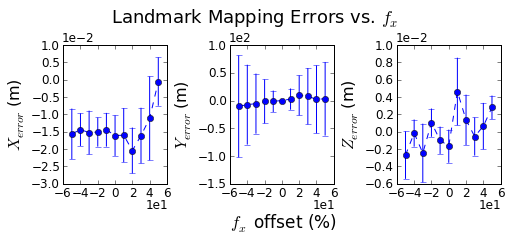
\includegraphics[width=7cm,keepaspectratio=true]{./Figures/SimulationFigures/Figure38.png}
  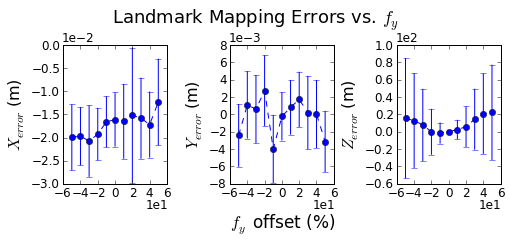
\includegraphics[width=7cm,keepaspectratio=true]{./Figures/SimulationFigures/Figure39.png}
  \caption{Feature mapping error statistic with variable $(f_x, f_y)$}
  \label{fig:simfig38-39}
\end{figure}

Plotting the feature mapping error against feature ground truth
position reveals how error in $(f_x, f_y)$ estimate impact on feature
position estimate. When $f_x$ estimate contains error, Y component of
feature position is determined by the feature's ground truth position
on X and Y components. The value of $Y_{error}$ is directly proportional
to the Y component of its ground truth position, with the error in
$f_x$ determines the function's slope. Same relation can be found for
$Z_{error}$ with $f_y$, and $Z_{ground truth}$.

% TODO simfig38-39:Merge these two into one, showing only the related.
%\begin{figure}[h]
%  \centering
%  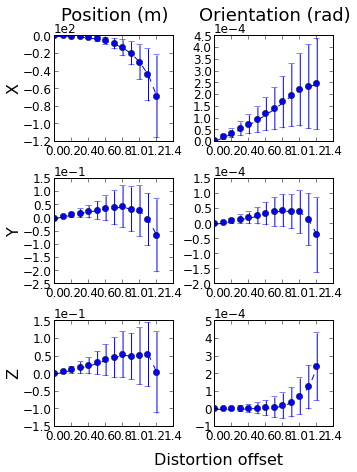
\includegraphics[width=10cm,keepaspectratio=true]{./Figures/SimulationFigures/Figure47.png}
%  \caption{Feature mapping error plotted against feature ground truth
%    for various $(f_x, f_y)$}
%  \label{fig:simfig47}
%\end{figure}
\begin{figure}[h]
  \centering
  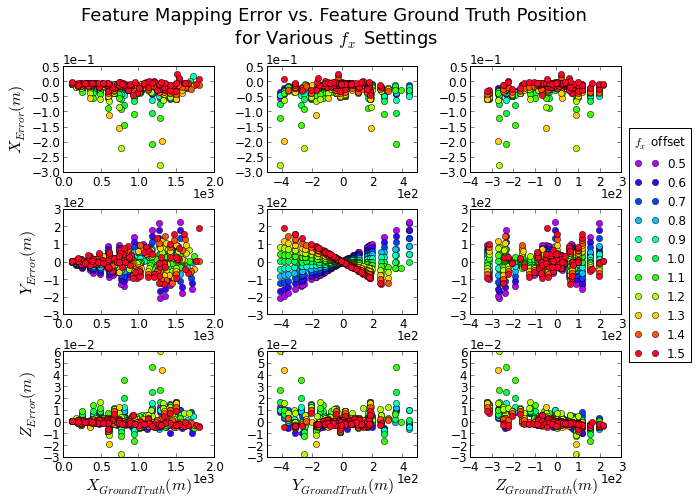
\includegraphics[width=7cm,keepaspectratio=true]{./Figures/SimulationFigures/Figure41.png}
  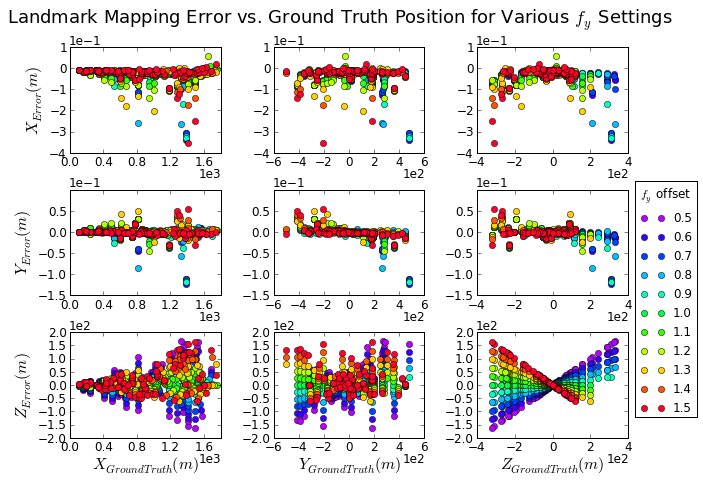
\includegraphics[width=7cm,keepaspectratio=true]{./Figures/SimulationFigures/Figure42.png}
  \caption{Feature mapping error plotted against feature ground truth
    for various $(f_x, f_y)$}
  \label{fig:simfig38-39}
\end{figure}

\FloatBarrier
\subsection{Effect from Distortion}

The CC\_EKF\_SLAM algorithm does not consider camera lens distortion
at this stage. Therefore, the simulation evaluate the effect of
distortion varying from 0\% to 150\% of the calibrated result to
evaluate the amount error resulted by ignoring the lens distortion. 

Figure \ref{fig:simfig48} (left) shows the UAS localization error for all
lens distortion setting. Ignoring the distortion brings significant
error into the UAS localization. UAS X position receives the most
impact with error up to 100 meters with increasing standard deviation.
Y and Z position shows less error, but standard deviation grows larger
with distortion offset.Figure \ref{fig:simfig48} (right) reveals the cause of
increasing standard deviation. The UAS position error was growing
larger with time. The UAS orientation estimates also experience error
increase going from maximum mean error of 5e-6 rad in low noise
simulation to 2.5e-4 rad. The standard deviation of orientation
estimates also increases with lens distortion offset. Similarly, the
orientation error vs. frame number plots show that the error amplitude
increase with time, although it fluctuates around zero. 

\begin{figure}[h]
  \centering
  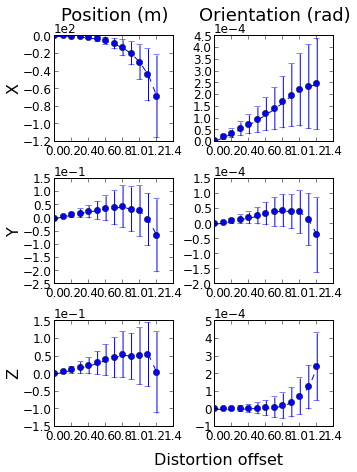
\includegraphics[width=5cm,keepaspectratio=true]{./Figures/SimulationFigures/Figure47.png}
  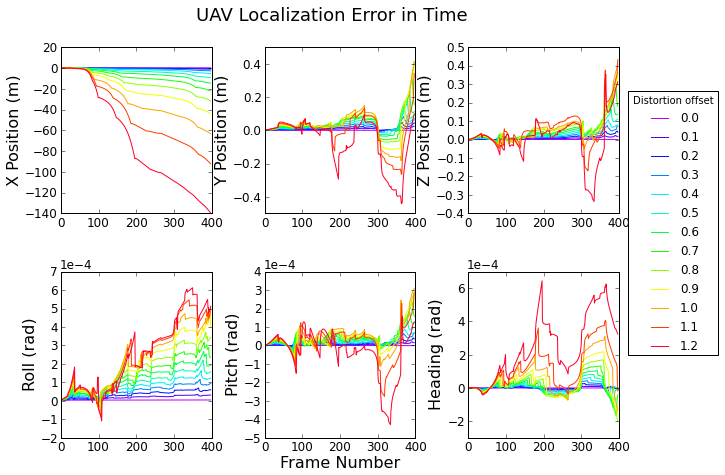
\includegraphics[width=9cm,keepaspectratio=true]{./Figures/SimulationFigures/Figure48.png}
  \caption{UAS localization error with lens distortion}
  \label{fig:simfig48}
\end{figure}

The feature mapping error statistic is shown in figure
\ref{fig:simfig45}. The X axis of feature position shows the most
error, with mean value reading -400 meters with distortion offset at
\%150. Y, and Z axis position has less mean error, but the standard
deviation is bigger. Plotting feature position error agains feature
ground truth coordinate (figure \ref{fig:simfig46}) shows that the
increasing standard deviation is due to the first order linear
relation between the Y (or Z) and the Y (or Z) axis of feature ground
truth coordinate, where distortion offset determine the slope of the
line. 

\begin{figure}[h]
  \centering
  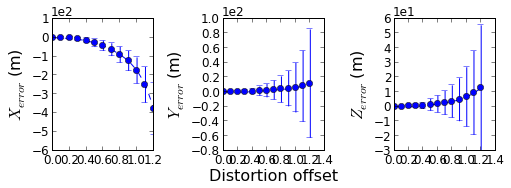
\includegraphics[width=10cm,keepaspectratio=true]{./Figures/SimulationFigures/Figure45.png}
  \caption{UAS localization error with lens distortion}
  \label{fig:simfig45}
\end{figure}

\begin{figure}[h]
  \centering
  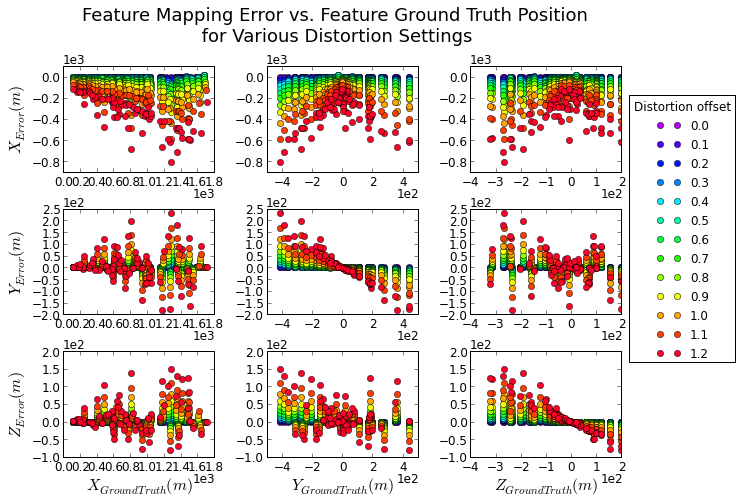
\includegraphics[width=10cm,keepaspectratio=true]{./Figures/SimulationFigures/Figure46.png}
  \caption{UAS localization error with lens distortion}
  \label{fig:simfig46}
\end{figure}

\FloatBarrier

\subsection{Effect from Image Resolution}

It is well known that higher resolution sensor will give more accuracy
to the estimate. To know how high a resolution is good enough for the
distance range that this work is targeting, a quantitive analysis is
necessary. The ideal case simulation is ran with various image
resolution setting, and the result is below (figure \ref{fig:simfig50}). 

\begin{figure}[h]
  \centering
  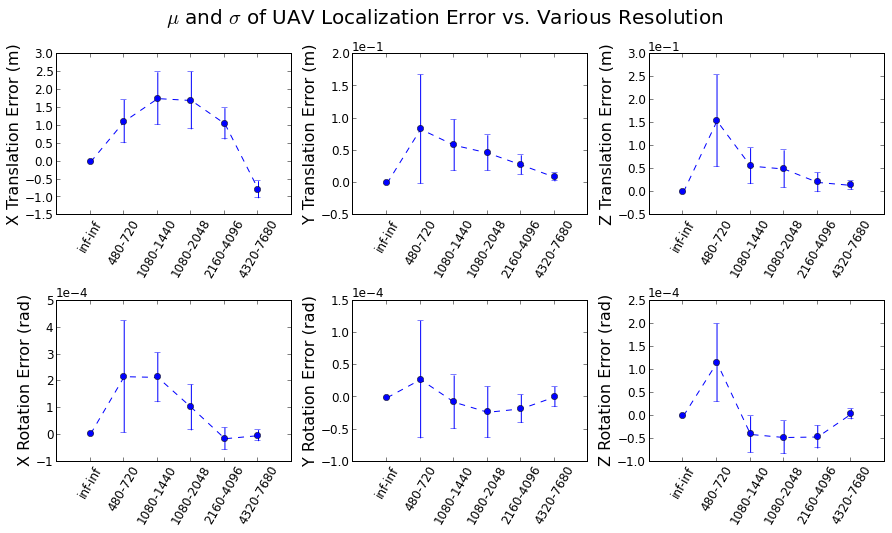
\includegraphics[width=10cm,keepaspectratio=true]{./Figures/SimulationFigures/Figure50.png}
  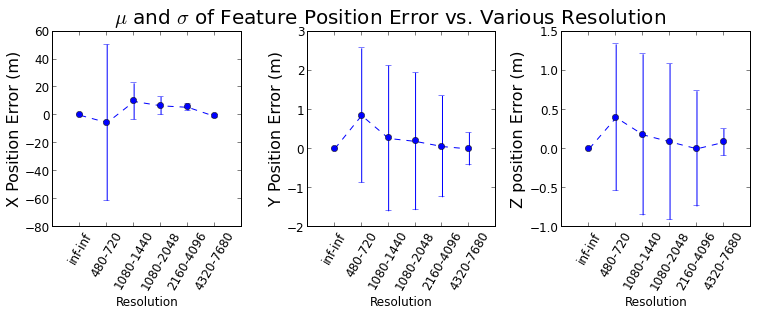
\includegraphics[width=10cm,keepaspectratio=true]{./Figures/SimulationFigures/Figure49.png}
  \caption{Error statistic for various image resolution}
  \label{fig:simfig50}
\end{figure}

This test confirmed that higher resolution the image sensor is, the
more accuracy it will bring. The most significant error is seen at
resolution 480x720 where the X axis of feature position error is +/-
150m. At one 720x1080, which is one step up of 480x720, the X axis
feature position error is hugely reduced to a few meters. For all
other parameters, improvement at each level of resolution increase is
nearly linear. This result suggests that to achieve reasonably good
accuracy for obstacle detection, a resolution of 720x1080 or higher is
preferred. 


%%% Local Variables:
%%% mode: latex
%%% TeX-master: "thesis"
%%% End:
